% VUT FIT 1MITAI
% TIN 2019/2020
% Project: Task 1
% Author: Vladimir Dusek, xdusek27
% Date: 15/10/2019
% File: xdusek27.tex

%%%%%%%%%%%%%%%%%%%%%%%%%%%%%%%%%%%%%%%%%%%%%%%%%%%%%%%%%%%%%%%%%%%%%

\documentclass[11pt, a4paper, titlepage]{article}
\usepackage[left=2cm, text={17cm, 24cm}, top=3cm]{geometry}
\usepackage[utf8]{inputenc}
\usepackage[czech]{babel}
\usepackage{pdfpages}
\usepackage{amssymb}
\usepackage{multicol}
\usepackage{enumitem}

\newcommand{\N}{\mathbb{N}_0}

\setlength\parindent{0pt}

%%%%%%%%%%%%%%%%%%%%%%%%%%%%%%%%%%%%%%%%%%%%%%%%%%%%%%%%%%%%%%%%%%%%%

\begin{document}

\begin{titlepage}
    \begin{center}
        \begin{figure}[htb]
            \centering
            
\includegraphics[width=0.85\hsize]{images/fitlogo.pdf}
        \end{figure}
        \vspace{\stretch{0.382}}
        {\Huge Teoretická informatika} \\
        \bigskip
        {\LARGE Úkol 1} \\
        \vspace{\stretch{0.618}}
    \end{center}
    {\Large \today \hfill Vladimír Dušek, xdusek27}
\end{titlepage}

%%%%%%%%%%%%%%%%%%%%%%%%%%%%%%%%%%%%%%%%%%%%%%%%%%%%%%%%%%%%%%%%%%%%%

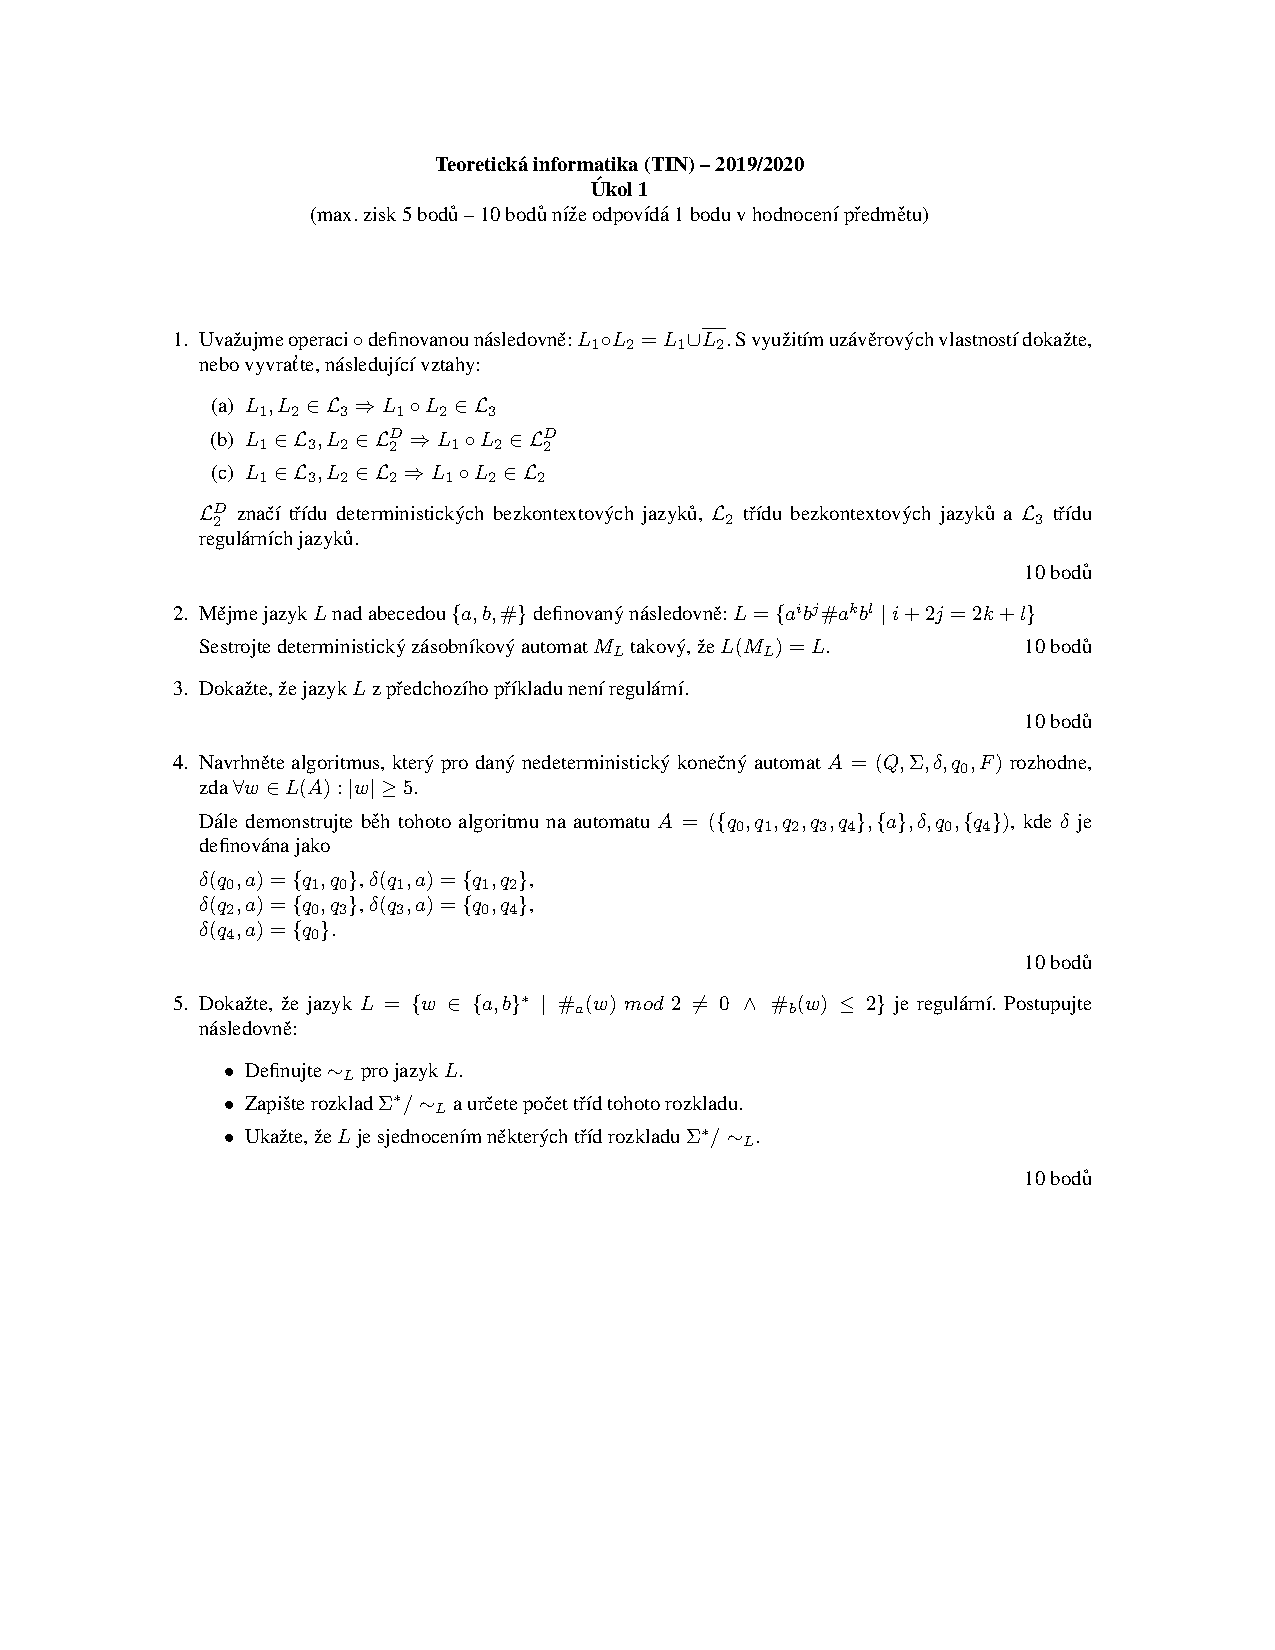
\includepdf{assignment.pdf}

%%%%%%%%%%%%%%%%%%%%%%%%%%%%%%%%%%%%%%%%%%%%%%%%%%%%%%%%%%%%%%%%%%%%%

\section*{Příklad 1}

\begin{enumerate}[label=\alph*)]

    \item
    Podle věty 3.22\footnote{\label{opora}http://www.fit.vutbr.cz/study/courses/TIN/public/Texty/TIN-studijni-text.pdf} plyne z definice regulárních množin a ekvivalence regulárních množin a regulárních jazyků, že třída regulárních jazyků je uzavřena vzhledem k operaci sjednocení.

    Na základě věty 3.23\textsuperscript{\ref{opora}} tvoří třída regulárních jazyků Booleovu algebru. Z její definice plyne, že Booleova algebra je uzavřena vzhledem k operaci doplněk.

    Jelikož $L_1, L_2 \in \mathcal{L}_3 \Rightarrow L_1 \cup \overline{L_2} \in \mathcal{L}_3$ a operace $\circ$ je definována jako $L_1 \circ L_2 = L_1 \cup \overline{L_2}$, tak i $L_1 \circ L_2 \in \mathcal{L}_3$.

    Zadané tvrzení platí.


    \item
    Podle věty 4.27\textsuperscript{\ref{opora}} jsou deterministické bezkontextové jazyky uzavřené vůči operaci doplněk a operaci průnik s regulárními jazyky.

    $L_1 \in \mathcal{L}_3 \Rightarrow \overline{L_1} \in \mathcal{L}_3$ a $L_2 \in \mathcal{L}_2^D \Rightarrow \overline{L_2} \in \mathcal{L}_2^D$

    $L_1 \in \mathcal{L}_3 \land L_2 \in \mathcal{L}_2^D \Rightarrow L_1 \cap L_2 \in \mathcal{L}_2^D$

    $\overline{L_1} \cap L_2 \in \mathcal{L}_2^D \Rightarrow \overline{\overline{L_1} \cap L_2} \in \mathcal{L}_2^D$

    Dle De Morganových zákonů platí: $\overline{\overline{L_1} \cap L_2} = L_1 \cup \overline{L_2}$

    Nyní můžeme říct, že $L_1 \in \mathcal{L}_3 \land L_2 \in \mathcal{L}_2^D \Rightarrow L_1 \cup \overline{L_2} \in \mathcal{L}_2^D$ a jelikož je operace $\circ$ definována jako $L_1 \circ L_2 = L_1 \cup \overline{L_2}$, tak i $L_1 \circ L_2 \in \mathcal{L}_2^D$.

    Zadané tvrzení platí.


    \item
    Podle věty 4.24\textsuperscript{\ref{opora}} nejsou bezkontextové jazyky uzavřeny vůči operaci doplněk a průnik.

    Podle De Morganových zákonů platí: $L_1 \cup \overline{L_2} = \overline{\overline{L_1} \cap L_2}$

    Z výše uvedeného vyplývá: $L_1 \in \mathcal{L}_3 \land L_2 \in \mathcal{L}_2 \Rightarrow L_1 \cup \overline{L_2} \notin \mathcal{L}_2$ a jelikož je operace $\circ$ definována jako $L_1 \circ L_2 = L_1 \cup \overline{L_2}$, tak i $L_1 \circ L_2 \notin \mathcal{L}_2$.

    Zadané tvrzení neplatí.

\end{enumerate}

\newpage

%%%%%%%%%%%%%%%%%%%%%%%%%%%%%%%%%%%%%%%%%%%%%%%%%%%%%%%%%%%%%%%%%%%%%

\section*{Příklad 2}

$M_L=(\{q_0, q_1, q_2, q_3, q_4, q_5\}, \{a, b, \#\}, \{Z, C\}, \delta, q_0, Z, \{q_5\})$

\begin{multicols}{3}

    $\delta(q_0, a, Z)=(q_0, CZ)$

    $\delta(q_0, a, C)=(q_0, CC)$

    $\delta(q_0, b, Z)=(q_1, CCZ)$

    $\delta(q_0, b, C)=(q_1, CCC)$

    $\delta(q_0, \#, Z)=(q_5, \epsilon)$

    $\delta(q_1, b, C)=(q_1, CCC)$

    $\delta(q_1, \#, C)=(q_2, C)$

    $\delta(q_2, a, C)=(q_3, \epsilon)$

    $\delta(q_2, b, C)=(q_4, \epsilon)$

    $\delta(q_3, \epsilon, C)=(q_2, \epsilon)$

    $\delta(q_4, b, C)=(q_4, \epsilon)$

    $\delta(q_4, \epsilon, Z)=(q_5, \epsilon)$

\end{multicols}

\bigskip

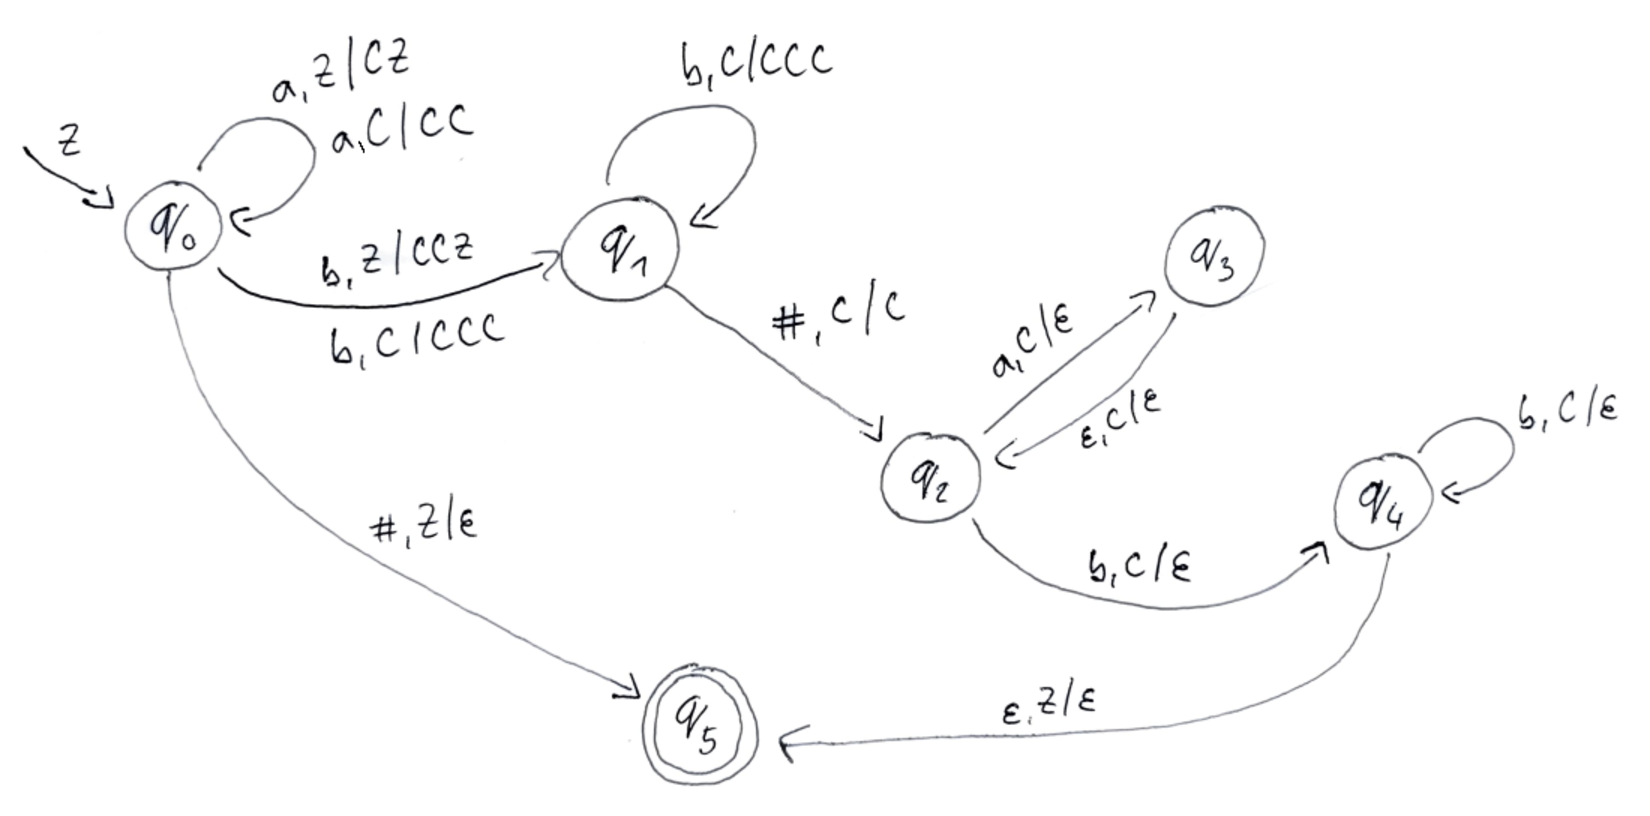
\includegraphics[page=1,scale=0.6]{images/priklad2-automat.pdf}

\newpage

%%%%%%%%%%%%%%%%%%%%%%%%%%%%%%%%%%%%%%%%%%%%%%%%%%%%%%%%%%%%%%%%%%%%%

\section*{Příklad 3}

\begin{itemize}

    \item Předpokládejme, že jazyk $L=\{a^i b^j \# a^k b^l \mid i+2j=2k+l \;;\; i,j,k,l \in \N \}$ nad abecedou $\Sigma = \{a, b, \#\}$ je regulární.

    \item Poté, podle Pumping lemma (věta 3.18\textsuperscript{\ref{opora}}) $\exists p>0 : \forall w \in L : |w| \ge p \Rightarrow \exists x, y, z \in \Sigma^* : w=xyz \land y \ne \epsilon \land |xy| \le p \land \forall m \in \N : xy^mz \in L$.

    \item Uvažujme libovolný parametr $p>0$ a pomocí něho zapišme nějaký řetězec $w \in L$ takový, aby splňoval výše uvedené. \begin{itemize}[label=$\circ$]
        \item $w=b^p \# a^p$
        \item $\forall p>0 : w \in L$
        \item $|w| \ge p \Leftrightarrow 2p + 1 \ge p$
    \end{itemize}

    \item Nyní uvažme všechna rozdělení řetězce $w$ na podřetězce $x$, $y$, $z$ takové, aby platily výše uvedené podmínky. Může nastat následující situace: \begin{itemize}[label=$\circ$]
        \item $x = b^{p-k-l}$
        \item $y = b^k$
        \item $z = b^l \# a^p \;;\; l \ge 0, k \ge 1$
    \end{itemize}

    \item Nyní pro všechna $m \ge 0$ musi platit, že $xy^mz \in L$ \begin{itemize}[label=$\circ$]
        \item Pro $m = 2$ má řetězec $w$ tvar $xy^2z = b^{p-k-l} b^{2k} b^l \# a^p$.
        \item Aby byl řetězec $w$ součástí jazyka $L$, muselo by platit, že počet $b$ před znakem $\#$ se rovná počtu $a$ za ním. Tedy rovnice $p-k-l+2k+l=p$. Ta má řešení $k=0$.
        \item $k=0$ je přímo ve sporu s předpokladem, že $k \ge 1$ a tím pádem $xy^2z \notin L$
        \end{itemize}

    \item Řetězec $w=b^p \# a^p$ není možné rozložit na takové podřetězce $x$, $y$, $z$, které by splňovaly podmínky Pumping lemma. Z~toho vyplývá, že jazyk $L$ není regulární.

\end{itemize}

\newpage

%%%%%%%%%%%%%%%%%%%%%%%%%%%%%%%%%%%%%%%%%%%%%%%%%%%%%%%%%%%%%%%%%%%%%

\section*{Příklad 4}

\subsection*{Návrh algoritmu}

\begin{itemize}

    \item \textbf{Vstup:} Nedeterministický konečný automat $A=(Q, \Sigma, \delta, q_0, F)$
    \item \textbf{Výstup:} True/False
    \item \textbf{Metoda:} \begin{enumerate}

        \item Pokud $\nexists w \in \Sigma^* : (q_0, w) \vdash^* (q_f, \epsilon)$, $q_f \in F$, tak $L(A)=\emptyset$, tvrzení $\forall w \in L(A) : |w| \ge 5$ neplatí a ukončeme provádění algoritmu.

        \item Sestavme množinu řetězců $W=\{w | w \in \Sigma^* \land |w| < 5\}$.

        \item Pokud $W=\emptyset$, tak tvrzení $\forall w \in L(A) : |w| \ge 5$ platí a ukončeme provádění algoritmu.

        \item Vyjměme libovolný řetězec $w$ z~množiny $W$.

        \item Pokud pro řetězec $w$ platí $(q_0, w) \vdash^* (q_f, \epsilon)$, $q_f \in F$, tak $\exists w \in L(A) : |w|<5$. Tvrzení $\forall w \in L(A) : |w| \ge 5$ tedy neplatí a ukončeme provádění algoritmu. Jinak pokračujme krokem 3.

    \end{enumerate}

\end{itemize}

\subsection*{Demonstrace běhu algoritmu}

\begin{multicols}{2}
    \begin{enumerate}

        \item Máme nedeterministický konečný automat $A$, viz zadání.
        \item Jelikož pro $w=aaaa$ platí $(q_0, w) \vdash^* (q_4, \epsilon)$, řetězec $w$ je přijímán automatem $A$ a jazyk $L(A) \neq \emptyset$.
        \item $W=\{\epsilon, a, aa, aaa, aaaa\}$.

        \item $W \neq \emptyset$.
        \item $w=\epsilon$.
        \item $(q_0, w) \nvDash^* (q_4, \epsilon)$.

        \item $W \neq \emptyset$ ($W=\{a, aa, aaa, aaaa\}$).
        \item $w=a$.
        \item $(q_0, w) \nvDash^* (q_4, \epsilon)$.

        \item $W \neq \emptyset$ ($W=\{aa, aaa, aaaa\}$).
        \item $w=aa$.
        \item $(q_0, w) \nvDash^* (q_4, \epsilon)$.

        \item $W \neq \emptyset$ ($W=\{aaa, aaaa\}$).
        \item $w=aaa$.
        \item $(q_0, w) \nvDash^* (q_4, \epsilon)$.

        \item $W \neq \emptyset$ ($W=\{aaaa\}$).
        \item $w=aaaa$.
        \item $(q_0, w) \vdash^* (q_4, \epsilon)$, tvrzení $\forall w \in L(A) : |w| \ge 5$ neplatí.

    \end{enumerate}
\end{multicols}

\newpage

%%%%%%%%%%%%%%%%%%%%%%%%%%%%%%%%%%%%%%%%%%%%%%%%%%%%%%%%%%%%%%%%%%%%%

\section*{Příklad 5}


$\forall u, v \in \Sigma^* : u \sim_L v \Leftrightarrow (\#_a(u)\;mod \ 2 = \#_a(v)\;mod \ 2) \land ((\#_b(u) > 2 \land \#_b(v) > 2) \lor (\#_b(u) = \#_b(v)))$

\bigskip


$\Sigma^* / \sim_L$:

$L_1 = \{ w \in \{a, b\}^* \mid \, \#_b(w) = 0 \land \#_a(w) \; mod \ 2 = 0 \}$

$L_2 = \{ w \in \{a, b\}^* \mid \, \#_b(w) = 0 \land \#_a(w) \; mod \ 2 = 1 \}$

$L_3 = \{ w \in \{a, b\}^* \mid \, \#_b(w) = 1 \land \#_a(w) \; mod \ 2 = 0 \}$

$L_4 = \{ w \in \{a, b\}^* \mid \, \#_b(w) = 1 \land \#_a(w) \; mod \ 2 = 1 \}$

$L_5 = \{ w \in \{a, b\}^* \mid \, \#_b(w) = 2 \land \#_a(w) \; mod \ 2 = 0 \}$

$L_6 = \{ w \in \{a, b\}^* \mid \, \#_b(w) = 2 \land \#_a(w) \; mod \ 2 = 1 \}$

$L_7 = \{ w \in \{a, b\}^* \mid \, \#_b(w) > 2 \land \#_a(w) \; mod \ 2 = 0 \}$

$L_8 = \{ w \in \{a, b\}^* \mid \, \#_b(w) > 2 \land \#_a(w) \; mod \ 2 = 1 \}$

\bigskip


$L = L_2 \cup L_4 \cup L_6$

\bigskip


Relace $\sim_L$ má konečný index (8) a jazyk $L$ je tvořen sjednocením některých tříd rozkladu ($L_2, L_4, L_6$). Podle Myhill-Nerodovy věty (věta 3.20\textsuperscript{\ref{opora}}), jsou tato tvrzení ekvivalentní s~tvrzením, že jazyk $L$ je přijímaný deterministickým konečným automatem. Každý jazyk přijímaný deterministickým konečným automat je regulární. Jazyk $L$ je regulární.

%%%%%%%%%%%%%%%%%%%%%%%%%%%%%%%%%%%%%%%%%%%%%%%%%%%%%%%%%%%%%%%%%%%%%

\end{document}
